\documentclass{beamer}

% To have the citation lists ordered by number.
\usepackage[nocompress]{cite}
\usepackage[utf8]{inputenc}
\usepackage{graphicx}
\usepackage[tight,TABTOPCAP]{subfigure}
\usepackage{amsmath}
\usepackage{amssymb}
\usepackage{amsfonts}
\usepackage{url}
\usepackage{xspace}

\usepackage{hyperref}

\usepackage{tikz}
\usetikzlibrary{calc}
\usetikzlibrary{shapes.symbols}
\usetikzlibrary{shapes}
\usepackage{color}


%%%%%%%%%% Tool Names %%%%%%%%%%%%
\newcommand{\flex}{\textsf{Flextic}\xspace}
\newcommand{\fisch}{\textsf{Fisch}\xspace}
\newcommand{\blind}{\textsf{Blind}\xspace}
\newcommand{\hadoop}{\textsf{Hadoop}\xspace}

%%%%%%%%%% tikz macro %%%%%%%%%%%%%%%
%\sched{idx}{start}{duration}{label}
\newcommand{\sched}[4]{
  \draw[fill=blue!30] (#2/4, #1 -0.3) rectangle +(#3/4 , 0.6);
  \node at (#2/4 + #3/8, #1) {\scriptsize #4};
}

\mode<presentation>
{
  \usetheme{Warsaw}
  %\usetheme{Frankfurt}
  % or ...

  %\setbeamercovered{transparent}
  % or whatever (possibly just delete it)
  %\setbeamertemplate{footline}[frame number]
  \useoutertheme{mysplit}
}
% Remove the navigation bar
\setbeamertemplate{navigation symbols}{}

\title[Static Scheduling in Clouds]{Static Scheduling in Clouds}

%\AtBeginSection[]
%{
%  \begin{frame}<beamer>
%    \frametitle{Outline}
%    \tableofcontents[currentsection,hideothersubsections]
%  \end{frame}
%}

\author[Damien Zufferey]{
  Thomas A.~Henzinger \and
  Anmol V. Singh \and
  Vasu Singh \and
  Thomas Wies \and
  \alert{Damien Zufferey}
}

%TODO some mention of HotCloud in the title slide ??

\institute{ IST Austria }
\date{June 14, 2011}

%-------------------------------------------------------------------------
\begin{document}

% Title
\frame[plain]{\titlepage}

\begin{frame}
  \frametitle{Motivation (1)}
  Cloud computing gives the \emph{illusion} of $\infty$ (virtual) resources.

  \vspace{2ex}
  
  Actually there is a finite amount of (physical) resources.

  \vspace{2ex}
  
  We would like to efficiently share those resources:
  \begin{enumerate}
  \item being able to distinguish high priority (serving customer \emph{now}) from low priority (batch) requests;
  \item schedule accordingly.
  \end{enumerate}
  
  \vspace{2ex}
  
  Therefore, we should be able to \alert{plan ahead} computations.

\end{frame}

\begin{frame}
  \frametitle{Motivation (2)}

  Dynamic Scheduling: use work queues, priorities, but limited.

  \vspace{2ex}
  
  Without knowledge of jobs, this is the best you can do.

  \vspace{1cm}
  
  We need to ask the user for:
  \begin{itemize}
  \item what kind of resources his job require;
  \item a deadline/priority for his job.
  \end{itemize}

  \vspace{2ex}
  
  In exchange we can give him an expected completion time.

  \vspace{1cm}

  We can also offer choice. (time is money.)
  
\end{frame}

\begin{frame}
  \frametitle{\flex Overview}
  \begin{figure}
    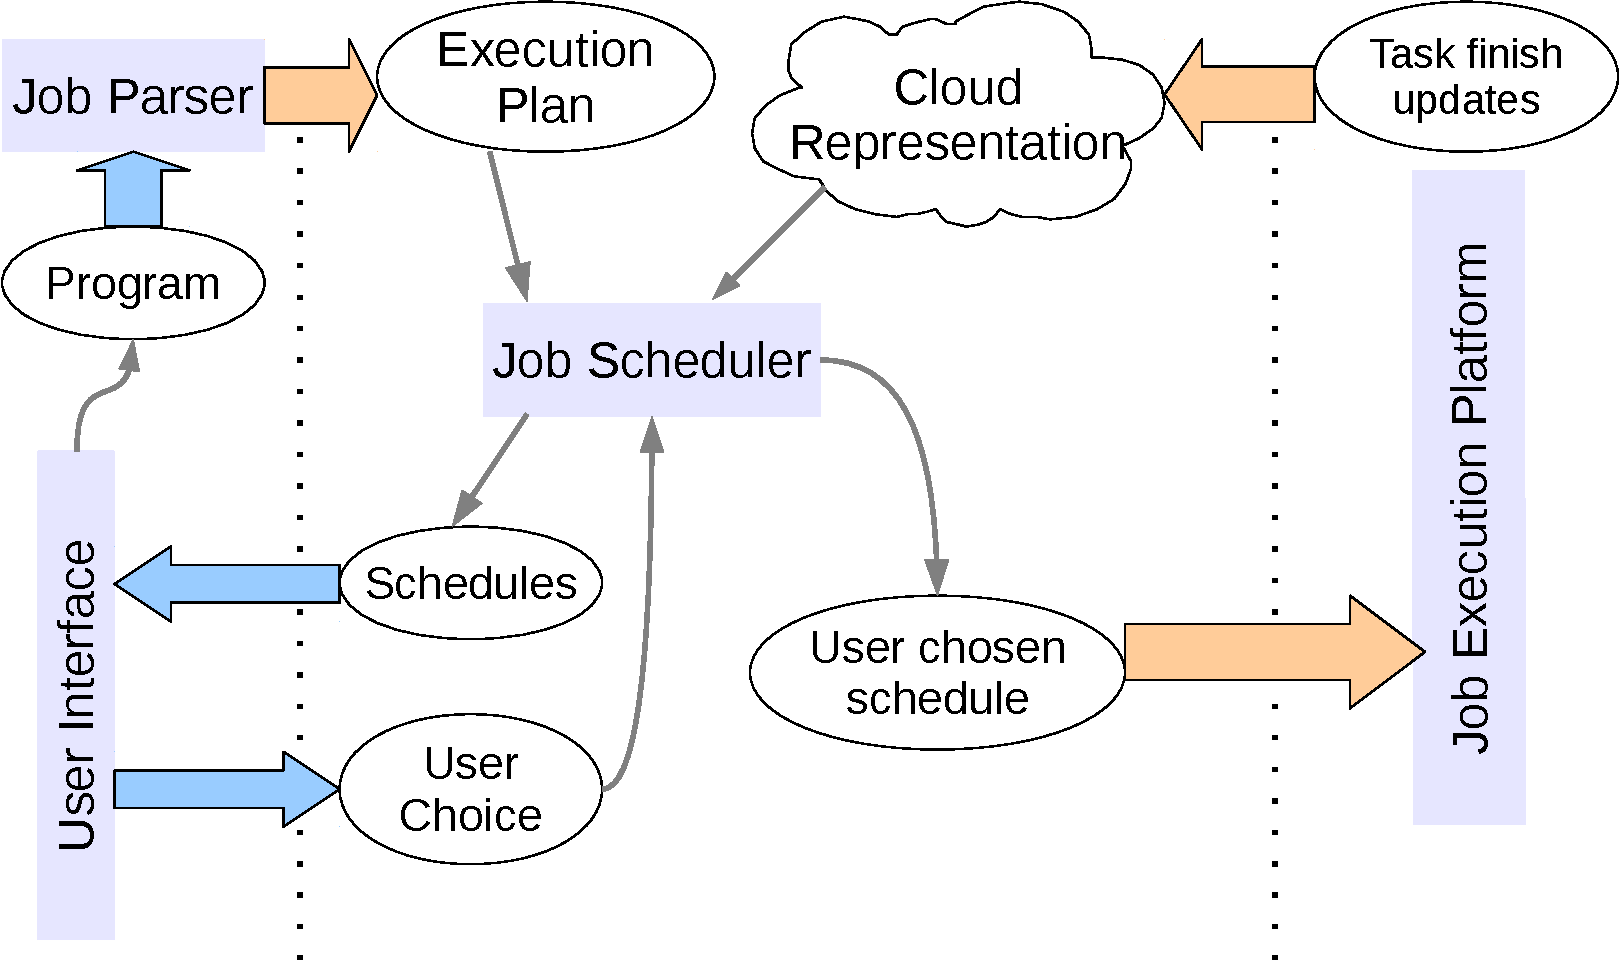
\includegraphics[scale=0.4]{overview}
  \end{figure}
\end{frame}

\begin{frame}
  \frametitle{Giving incentive to plan in advance}

  The scheduler returns not one but many possible schedules with different finish times.

  Use a pricing model to associate a cost to the schedules.

  Include the ``scheduling difficulty'' in the cost, give a discount to schedule with later finish time.

  \begin{figure}
    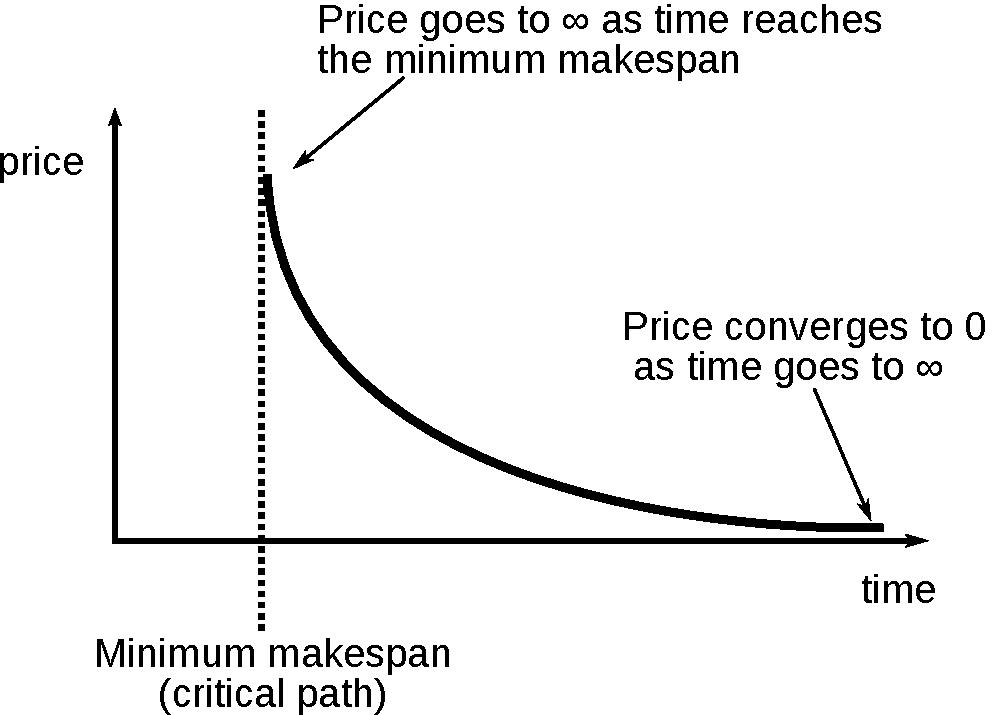
\includegraphics[scale=0.3]{price_curve}
  \end{figure}

  Problem: static scheduling is \emph{hard}.

  Only possible if the scheduler can handle the work load.

\end{frame}

\begin{frame}
  \frametitle{Jobs Model}
  \begin{figure}
    \centering
    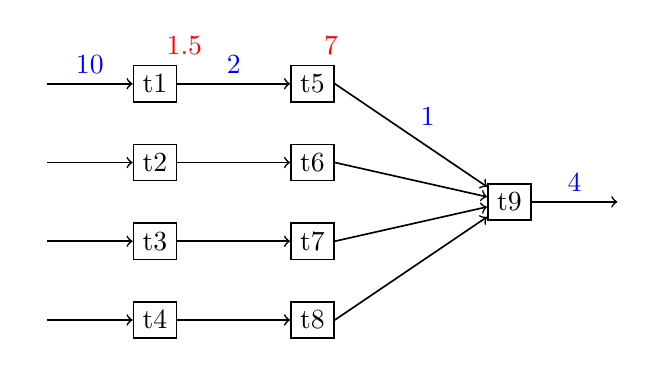
\begin{tikzpicture}[->,semithick]
      \node (d1) at (0,1.5)   {};
      \node (d2) [below of=d1]     {};
      \node (d3) [below of=d2]   {};
      \node (d4) [below of=d3]   {};
      \node[draw,label=85:\textcolor{red}{1.5}] (t1) [right=5mm, right of=d1]  {t1};
      \node[draw] (t2) [below of=t1]  {t2};
      \node[draw] (t3) [below of=t2]  {t3};
      \node[draw] (t4) [below of=t3]  {t4};
      \node[draw,label=85:\textcolor{red}{7}] (t5) [right=1cm, right of=t1]  {t5};
      \node[draw] (t6) [below of=t5]  {t6};
      \node[draw] (t7) [below of=t6]  {t7};
      \node[draw] (t8) [below of=t7]  {t8};
      \node[draw] (t9) at (6,0)    {t9};
      \node (d9) [right=5mm, right of=t9] {};
      \path (d1) edge node [above] {\textcolor{blue}{10}} (t1);
      \path (d2) edge (t2);
      \path (d3) edge (t3);
      \path (d4) edge (t4);
      \path (t1) edge node [above] {\textcolor{blue}{2}} (t5);
      \path (t2) edge (t6);
      \path (t3) edge (t7);
      \path (t4) edge (t8);
      \path (t5.east) edge node [above right] {\textcolor{blue}{1}} (t9);
      \path (t6.east) edge (t9);
      \path (t7.east) edge (t9);
      \path (t8.east) edge (t9);
      \path (t9) edge node [above] {\textcolor{blue}{4}}(d9);
    \end{tikzpicture}
  \end{figure}

  \begin{itemize}
  \item A Job is a directed acyclic task (DAG) of tasks.
  \item Node are marked with \textcolor{red}{worst case duration}.
  \item Edges are marked with \textcolor{blue}{data transfer}.
  \item duration and data can be parametric in the input.
  \end{itemize}
\end{frame}

\begin{frame}
  \frametitle{Parametric Jobs}
  \begin{figure}
    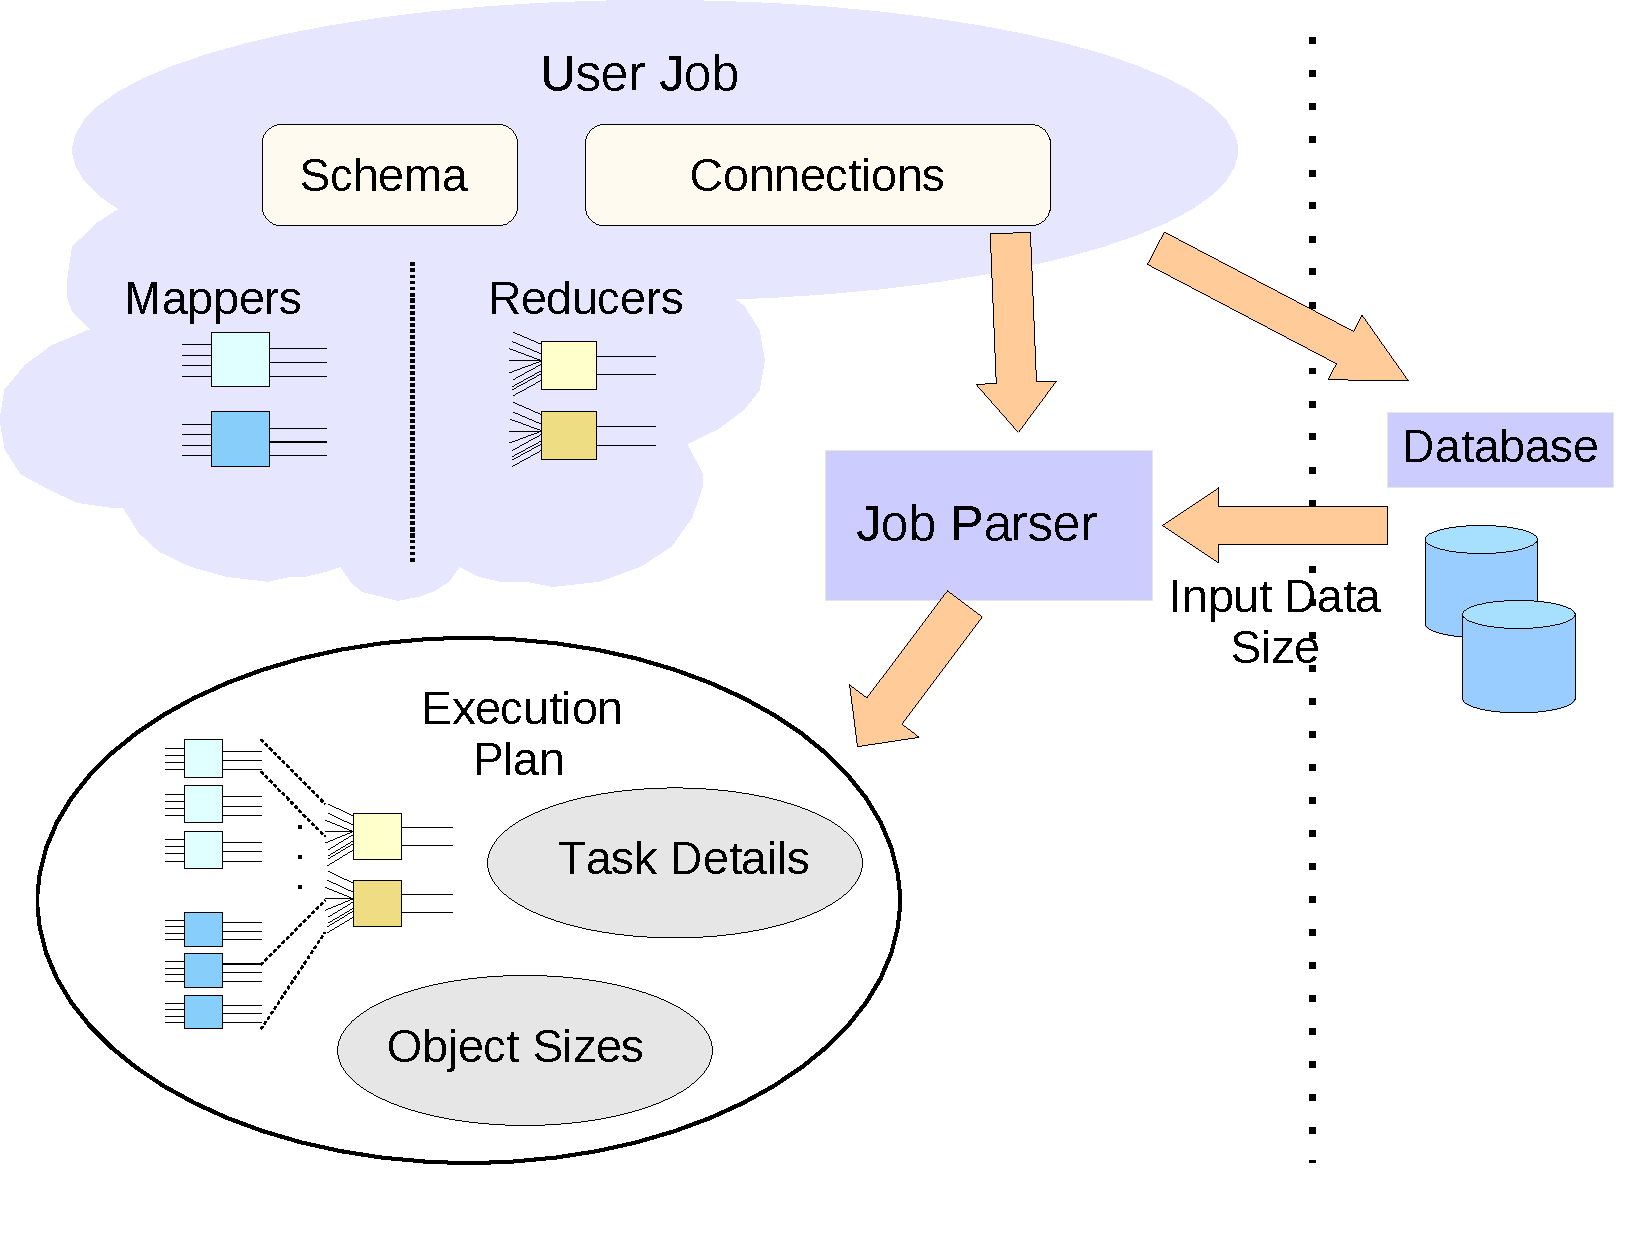
\includegraphics[scale=0.3]{parser1}
  \end{figure}
\end{frame}

\begin{frame}
  \frametitle{Infrastructure Model}

  \begin{figure}
    \centering
    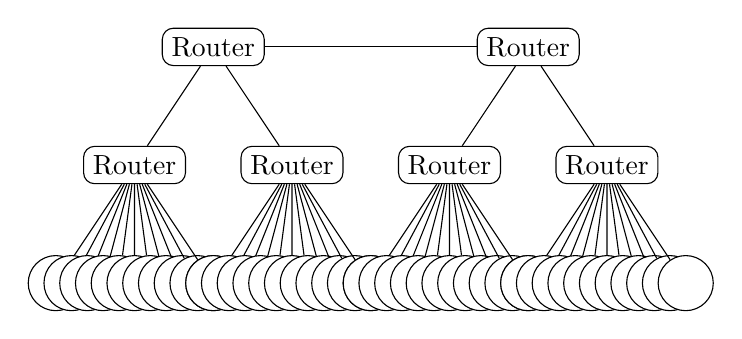
\begin{tikzpicture}
      \node[rounded corners,draw] (router1) at (1,3) {Router};
      \node[rounded corners,draw] (router2) at (5,3) {Router};
      \node[rounded corners,draw] (r1) at (0,1.5) {Router};
      \node[rounded corners,draw] (r2) at (2,1.5) {Router};
      \node[rounded corners,draw] (r3) at (4,1.5) {Router};
      \node[rounded corners,draw] (r4) at (6,1.5) {Router};
      \path (router1) edge (router2);
      \path (router1) edge (r1);
      \path (router1) edge (r2);
      \path (router2) edge (r3);
      \path (router2) edge (r4);
      \foreach \i in {0,0.2,...,2} {
        \node[draw,circle,fill=white,minimum height=7mm] (p1) at (-1 + \i, 0) {};
        \path (p1) edge (r1);
      }
      \foreach \i in {0,0.2,...,2} {
        \node[draw,circle,fill=white,minimum height=7mm] (p1) at (1 + \i, 0) {};
        \path (p1) edge (r2);
      }
      \foreach \i in {0,0.2,...,2} {
        \node[draw,circle,fill=white,minimum height=7mm] (p1) at (3 + \i, 0) {};
        \path (p1) edge (r3);
      }
      \foreach \i in {0,0.2,...,2} {
        \node[draw,circle,fill=white,minimum height=7mm] (p1) at (5 + \i, 0) {};
        \path (p1) edge (r4);
      }
    \end{tikzpicture}
  \end{figure}

  Datacenter as a tree-like graph:
  \begin{itemize}
  \item internal nodes are router;
  \item leaves are compute nodes (computation speed);
  \item edges specifies the bandwidth.
  \end{itemize}

\end{frame}

\begin{frame}
  \frametitle{Scheduling Large Jobs using Abstraction [EuroSys 2011]}
  Assumption: job and infrastructure \alert{regularity} 

  \vspace{1ex}

  Idea: regularity makes large scale scheduling feasible

  \vspace{1ex}

  How: Using abstraction techniques
  \begin{figure}
    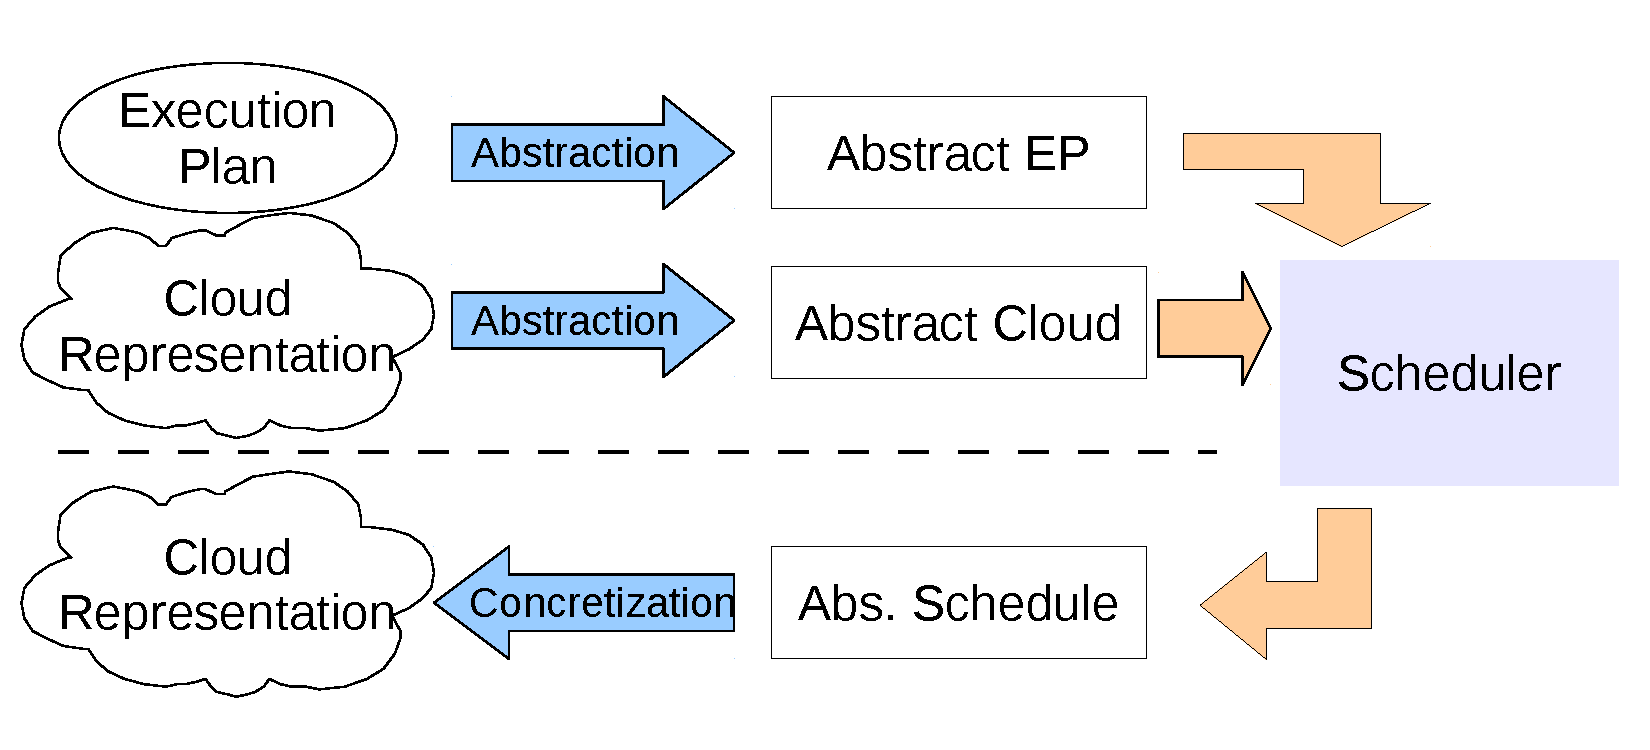
\includegraphics[scale=0.35]{abs_scheduling}
  \end{figure}
\end{frame}

\begin{frame}
  \frametitle{Abstraction for jobs:}

  Group independent tasks as per a topological sort.
  Merge them into an abstract task.

  \begin{figure}
    \centering
    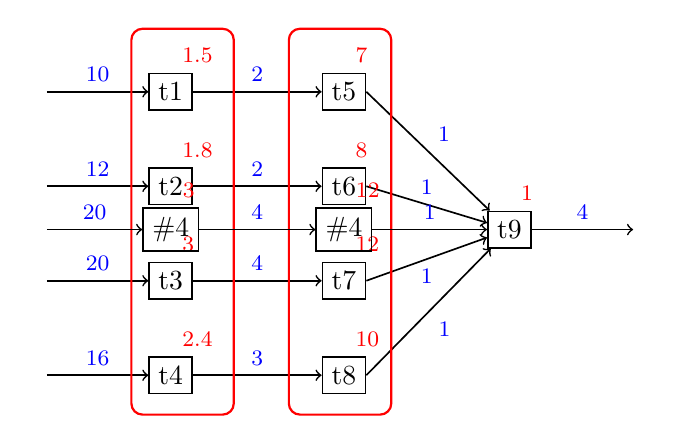
\begin{tikzpicture}[->,semithick, node distance=12mm]
      \node[draw,label=85:\textcolor{red}{\footnotesize 1}] (t9) at (6,-0.25)    {t9};
      \node (d9) [right=5mm, right of=t9] {};
      \path (t9) edge node [above] {\textcolor{blue}{\footnotesize 4}}(d9);
      \visible<1,2>{
      \node (d1) at (0,1.5)     {};
      \node (d2) [below of=d1]  {};
      \node (d3) [below of=d2]  {};
      \node (d4) [below of=d3]  {};
      \node[draw,label=85:\textcolor{red}{\footnotesize 1.5}] (t1) [right=5mm, right of=d1]  {t1};
      \node[draw,label=85:\textcolor{red}{\footnotesize 1.8}] (t2) [below of=t1]  {t2};
      \node[draw,label=85:\textcolor{red}{\footnotesize   3}] (t3) [below of=t2]  {t3};
      \node[draw,label=85:\textcolor{red}{\footnotesize 2.4}] (t4) [below of=t3]  {t4};
      \node[draw,label=85:\textcolor{red}{\footnotesize  7}] (t5) [right=1cm, right of=t1]  {t5};
      \node[draw,label=85:\textcolor{red}{\footnotesize  8}] (t6) [below of=t5]  {t6};
      \node[draw,label=85:\textcolor{red}{\footnotesize 12}] (t7) [below of=t6]  {t7};
      \node[draw,label=85:\textcolor{red}{\footnotesize 10}] (t8) [below of=t7]  {t8};
      \path (d1) edge node [above] {\textcolor{blue}{\footnotesize 10}} (t1);
      \path (d2) edge node [above] {\textcolor{blue}{\footnotesize 12}} (t2);
      \path (d3) edge node [above] {\textcolor{blue}{\footnotesize 20}} (t3);
      \path (d4) edge node [above] {\textcolor{blue}{\footnotesize 16}} (t4);
      \path (t1) edge node [above] {\textcolor{blue}{\footnotesize 2}} (t5);
      \path (t2) edge node [above] {\textcolor{blue}{\footnotesize 2}} (t6);
      \path (t3) edge node [above] {\textcolor{blue}{\footnotesize 4}} (t7);
      \path (t4) edge node [above] {\textcolor{blue}{\footnotesize 3}} (t8);
      \path (t5.east) edge node [above right] {\textcolor{blue}{\footnotesize 1}} (t9);
      \path (t6.east) edge node [above ] {\textcolor{blue}{\footnotesize 1}} (t9);
      \path (t7.east) edge node [below ] {\textcolor{blue}{\footnotesize 1}} (t9);
      \path (t8.east) edge node [below right] {\textcolor{blue}{\footnotesize 1}} (t9);
      \visible<2>{
        \draw[rounded corners,red,thick] (1.2,2.3) rectangle +(1.3,-4.9);
        \draw[rounded corners,red,thick] (3.2,2.3) rectangle +(1.3,-4.9);
      }
      }
      \visible<3>{
      \node (d22) at (0,-0.25)     {};
      \node[draw,label=85:\textcolor{red}{\footnotesize 3}] (t22) [right=5mm, right of=d22]  {\#4};
      \node[draw,label=85:\textcolor{red}{\footnotesize  12}] (t62) [right=1cm, right of=t22]  {\#4};
      \path (d22) edge node [above] {\textcolor{blue}{\footnotesize 20}} (t22);
      \path (t22) edge node [above] {\textcolor{blue}{\footnotesize 4}} (t62);
      \path (t62.east) edge node [above] {\textcolor{blue}{\footnotesize 1}} (t9);
      }
    \end{tikzpicture}
  \end{figure}

\end{frame}

\begin{frame}
  \frametitle{Abstraction for infrastructure:}

  Merge nodes to according to network topology:

  \begin{figure}
    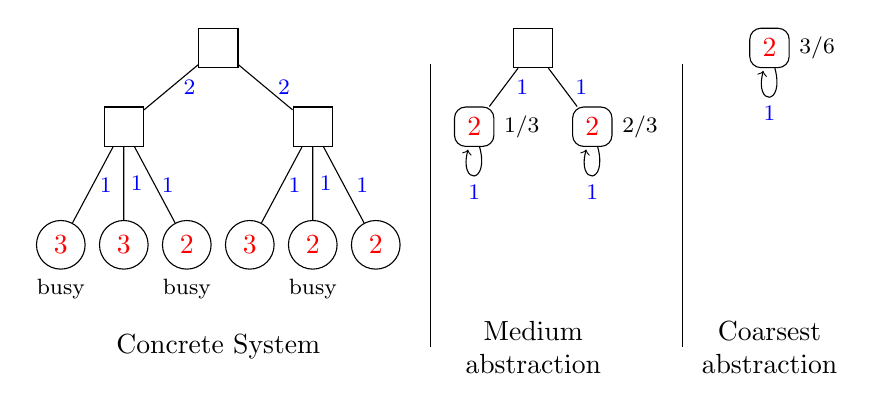
\begin{tikzpicture}[
        router/.style={draw, rectangle,minimum width=5mm, minimum height=5mm},
        machine/.style={draw, circle, minimum width=5mm, minimum height=5mm},
        abstract/.style={draw, rectangle, rounded corners, minimum width=5mm, minimum height=5mm}
      ]

    \begin{scope}[ yshift=0mm, xshift=0mm,
        level 1/.style={sibling distance=24mm, level distance=1cm},
        level 2/.style={sibling distance=8mm, level distance=1.5cm}
      ]
    \node[router] {}
      child {
        node[router] {}
        child {
          node[machine,label=below:{\footnotesize busy}] {\textcolor{red}{3}}
          edge from parent node [right=-1pt] {\footnotesize \textcolor{blue}{1}}
        }
        child {
          node[machine] {\textcolor{red}{3}}
          edge from parent node [right=-1pt] {\footnotesize \textcolor{blue}{1}}
        }
        child {
          node[machine,label=below:{\footnotesize busy}] {\textcolor{red}{2}}
          edge from parent node [right=-1pt] {\footnotesize \textcolor{blue}{1}}
        }
        edge from parent node [right=1pt] {\footnotesize \textcolor{blue}{2}}
      }
      child {
        node[router] {}
        child {
          node[machine] {\textcolor{red}{3}}
          edge from parent node [right=-1pt] {\footnotesize \textcolor{blue}{1}}
        }
        child {
          node[machine,label=below:{\footnotesize busy}] {\textcolor{red}{2}}
          edge from parent node [right=-1pt] {\footnotesize \textcolor{blue}{1}}
         }
        child {
          node[machine] {\textcolor{red}{2}}
          edge from parent node [right=1pt] {\footnotesize \textcolor{blue}{1}}
        }
        edge from parent node [right=1pt] {\footnotesize \textcolor{blue}{2}}
      };
    \end{scope}

    \begin{scope}[ yshift=0mm, xshift=40mm,
        level 1/.style={sibling distance=15mm, level distance=1cm} ]
    \node[router] {}
      child {
        node[abstract,label=right:{\footnotesize $1/3$}] (l1) {\textcolor{red}{2}}
        edge from parent node [right=1pt] {\footnotesize \textcolor{blue}{1}}
      }
      child {
        node[abstract,label=right:{\footnotesize $2/3$}] (l2) {\textcolor{red}{2}}
        edge from parent node [right=1pt] {\footnotesize \textcolor{blue}{1}}
      };
      \draw (l1) edge [loop below] node {\footnotesize \textcolor{blue}{1}} (l1);
      \draw (l2) edge [loop below] node {\footnotesize \textcolor{blue}{1}} (l2);
    \end{scope}

    \begin{scope}[ yshift=0mm, xshift=70mm]
    \node[abstract,label=right:{\footnotesize $3/6$}] (l3) {\textcolor{red}{2}};
    \draw (l3) edge [loop below] node {\footnotesize \textcolor{blue}{1}} (l3);
    \end{scope}

    \node at (0,-3.8) {Concrete System};
    \draw (2.7,-0.2) -- (2.7,-3.8);
    \node[text width=2cm,text centered] at (4,-3.8) {Medium abstraction};
    \draw (5.9,-0.2) -- (5.9,-3.8);
    \node[text width=2cm,text centered] at (7,-3.8) {Coarsest abstraction};

    \end{tikzpicture}
  \end{figure}
\end{frame}

\begin{frame}
  \frametitle{ Experiments: compared to \hadoop }

  Caution: static scheduling alone will not work.
  \begin{itemize}
  \item Task duration are conservative estimates;
  \item Variability of the performance of the compute node.
  \end{itemize}
  We use static scheduling with backfilling.

  \vfill

  \begin{figure}
    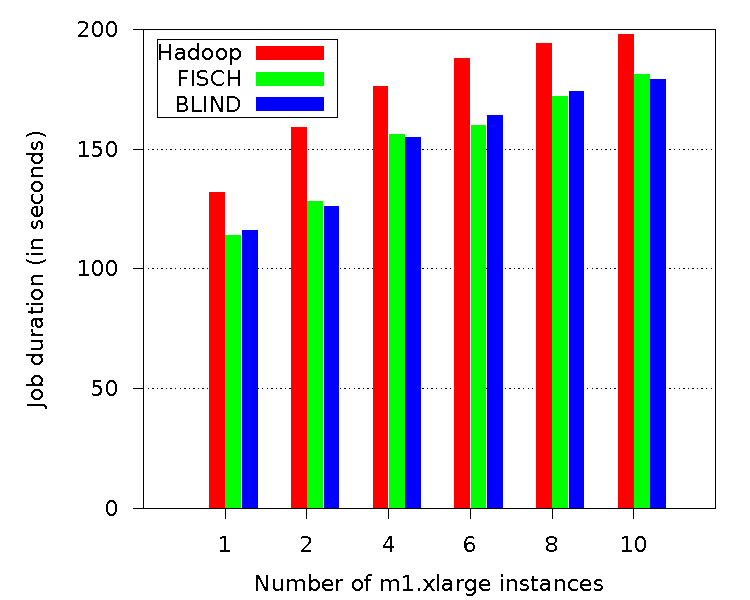
\includegraphics[scale=0.4]{comp_hadoop_1}
    \hspace{1ex}
    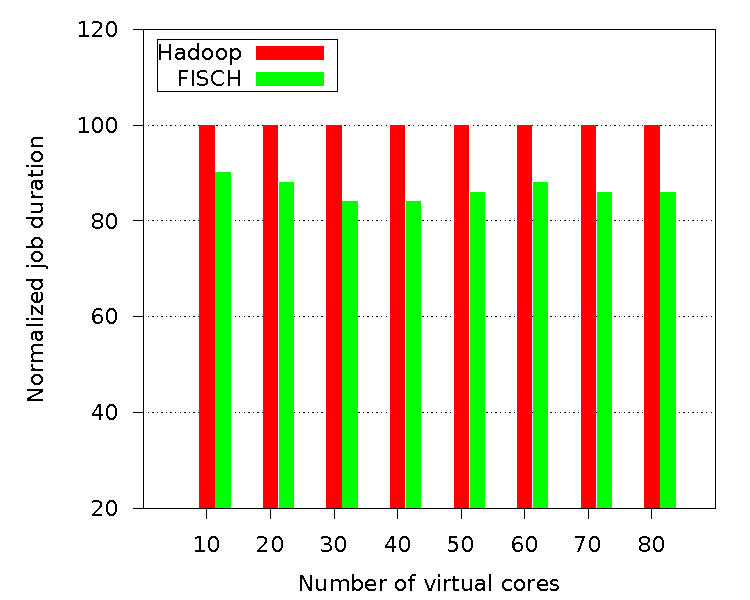
\includegraphics[scale=0.4]{comp_hadoop_2}
  \end{figure}
  
  \vfill

  \begin{itemize}
  \item The jobs are MapReduce jobs doing image transformation.
  \item Hadoop streaming version 0.19.0
  \end{itemize}

\end{frame}

%\section*{Conclusion}
\begin{frame}
\begin{center}
\Huge
Questions ?
\end{center}
\end{frame}


\end{document}
